\hypertarget{egyeni-es-kozossegi-szempontok}{%
\section{Egyéni és közösségi
szempontok}\label{egyeni-es-kozossegi-szempontok}}

\begin{figure}
\centering
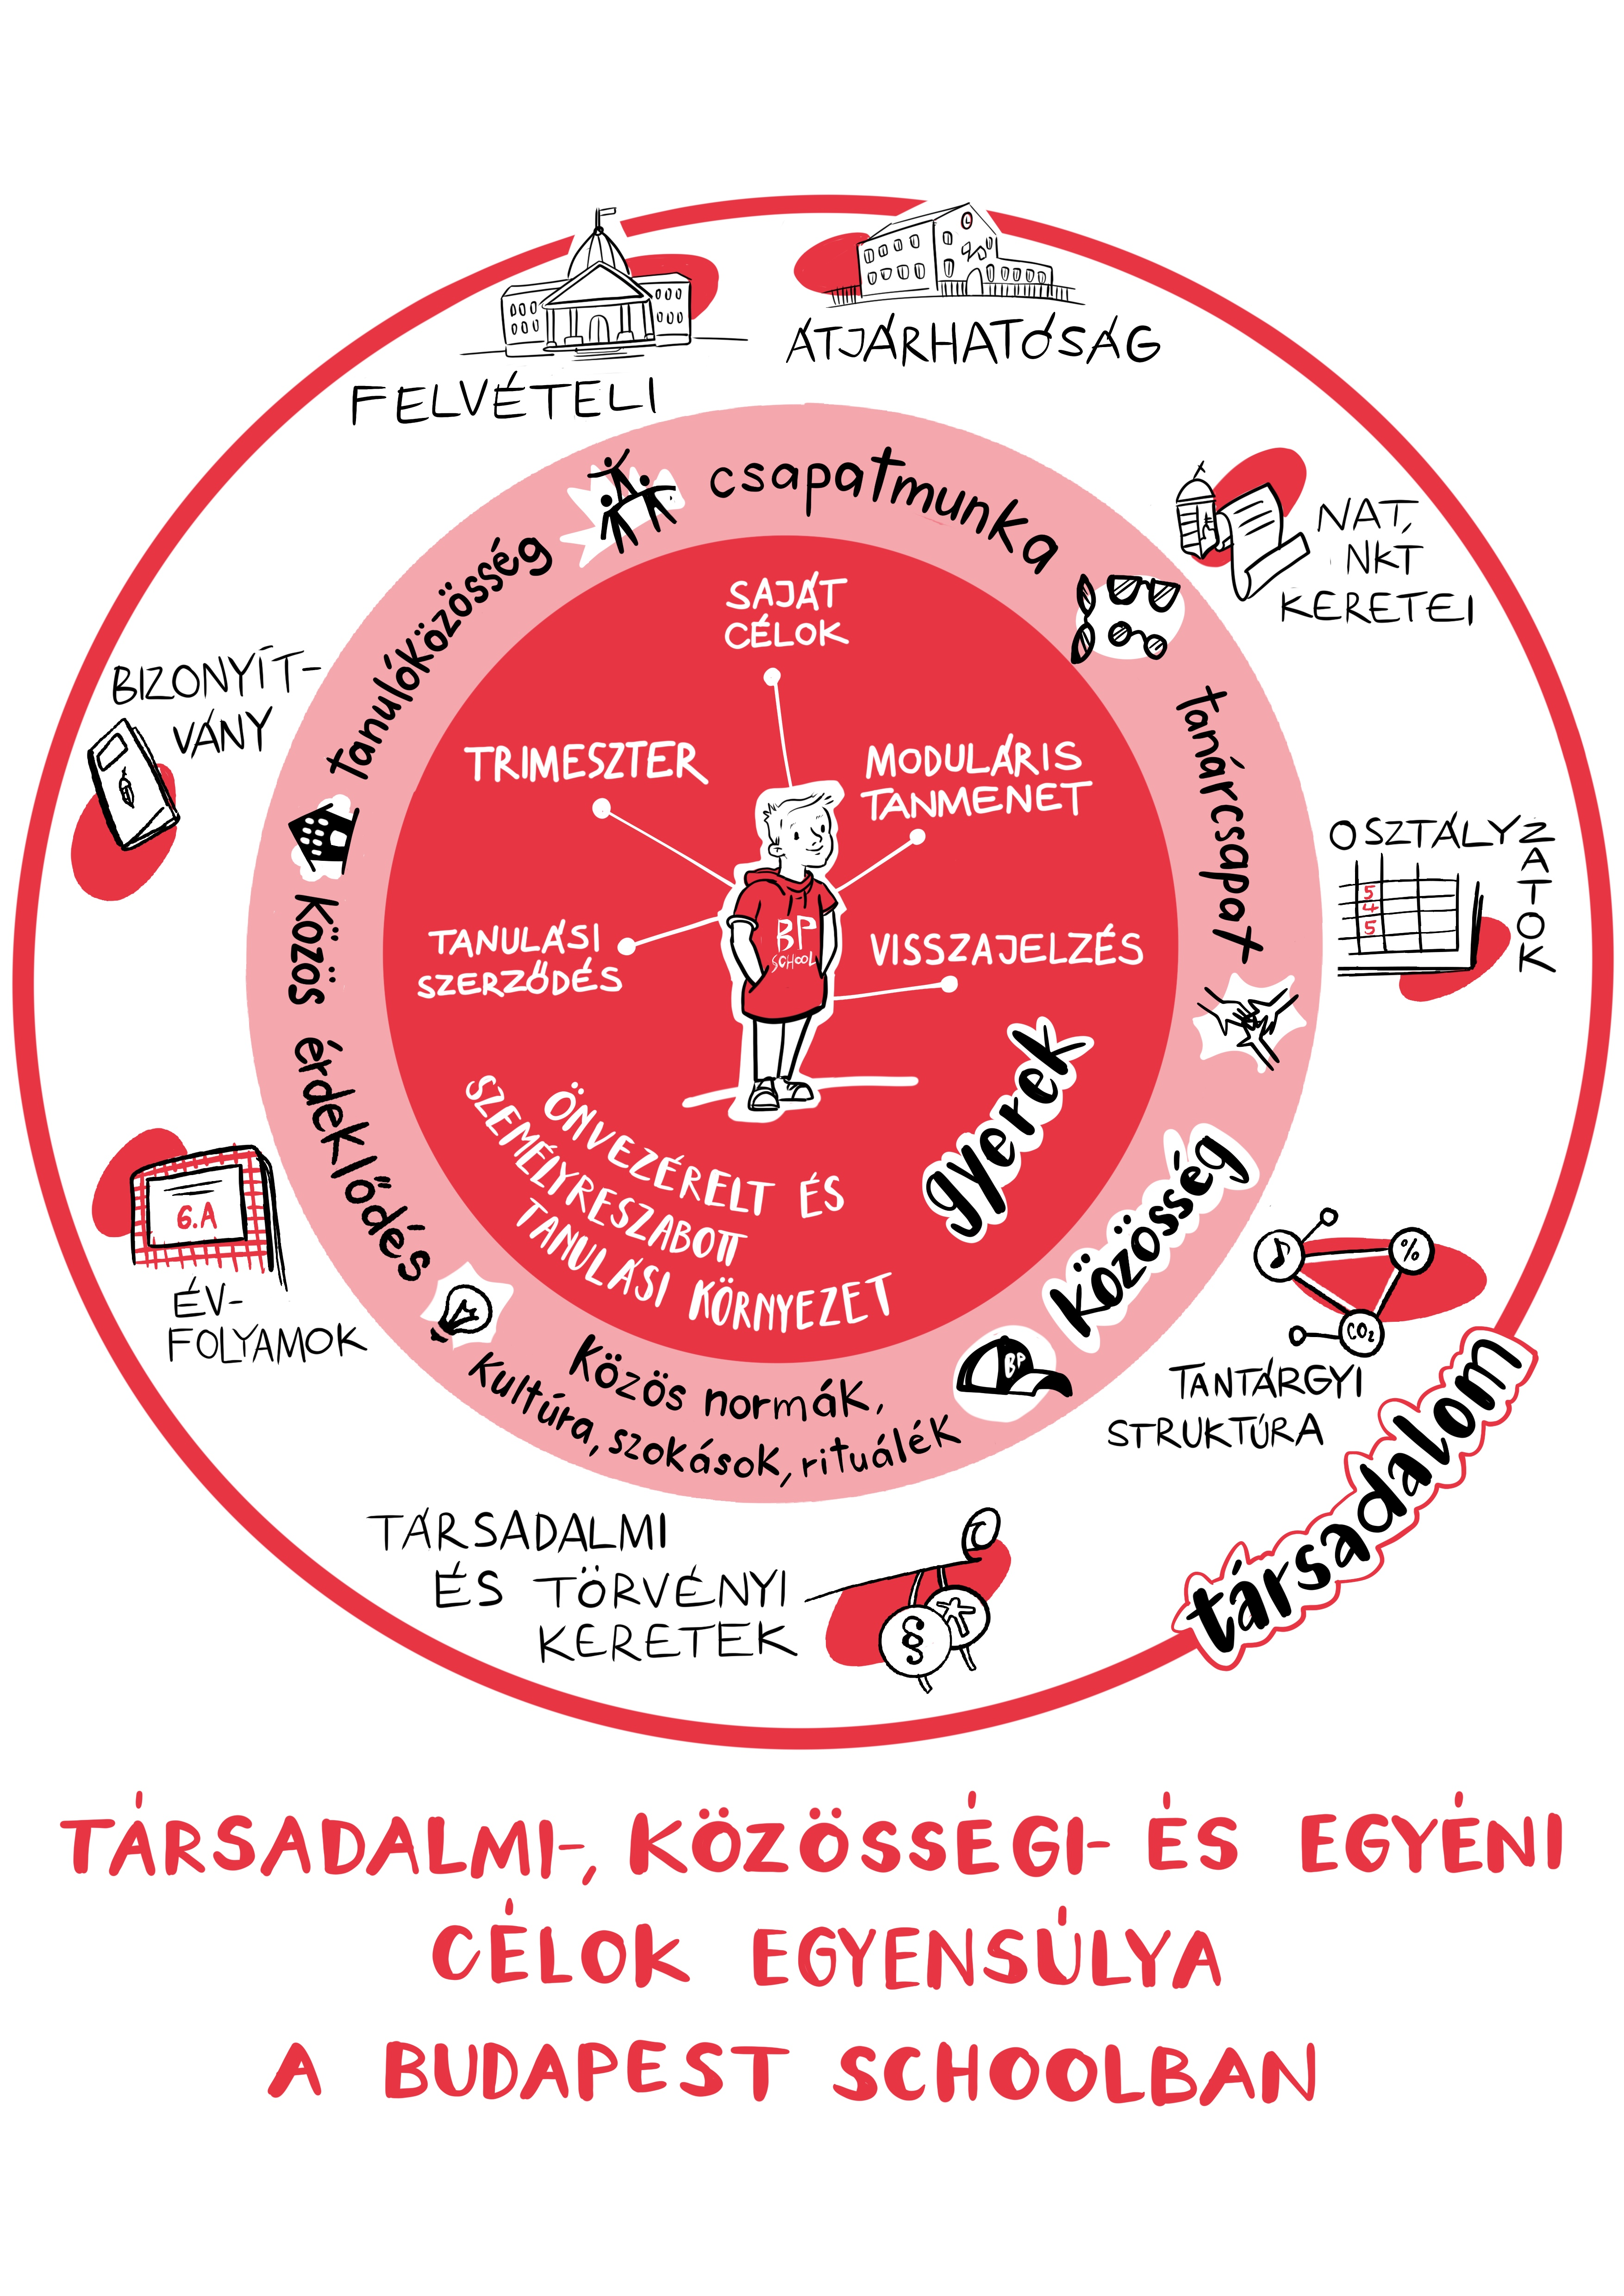
\includegraphics{pics/celok_egyensulya.jpg}
\caption{Egyéni és közösségi szempontok a Budapest School iskolában.}
\end{figure}

A Budapest School modellben az iskolának két rétege van. A gyerek
igényeire gyorsan reagáló tanulóközösség egy burok a gyerek körül. Ezt a
gyermekközpontú réteget veszi körül a társadalomhoz való kapcsolódást
biztosító külső réteg.

A belső burokban a Budapest School Modell a tanulás folyamatát
szabályozza, a \emph{Mit tanulunk?} kérdés helyett a \emph{Hogyan
szervezzük meg a tanulást?} kérdésre ad választ. A tanulás során a
gyerekek a Budapest School Modellben részletezett módon az
érdeklődésüknek megfelelően specifikus tanulási egységeket, vagyis
modulokat végeznek el, melyek eredményeit a saját portfóliójukban
gyűjtik össze. Így a gyerekek tanulási útja a portfólió fejlődésével
nyomon követhető, és a portfólió tartalma alapján megállapítható a
gyerek aktuális tudása, képessége. Az iskola fő funkciója emellett
mindvégig az aktív tanulás, saját fejlődésük kereteinek megtalálása, a
folyamatosan újragondolt saját célok állítása, és e célok irányába
történő haladás marad.

A belső réteg a személyre szabott és önvezérelt tanuláshoz szükséges
célkitűzés-tervezés, tanulás, és az arra történő reflektálás módját írja
le, vagyis a tanulás folyamatát rögzíti, míg annak pontos tartalmában
szabadságot enged.

\hypertarget{nat-hoz-a-kerettantervekhez-es-mas-kovetelmenyekhez-valo-kapcsolodas}{%
\subsection{A NAT-hoz, a kerettantervekhez és más követelményekhez\\ való
kapcsolódás}\label{nat-hoz-a-kerettantervekhez-es-mas-kovetelmenyekhez-valo-kapcsolodas}}

Ezt a szabadságot keretezik a társadalmi normák és jogszabályi
elvárások, hogy biztosítva legyen a gyerekek boldogulása a BPS iskolán
kívül is. Ezért a BPS modell alapján működő iskola programja a magyar
Nemzeti alaptanterv {\autocite{Nat2020}}, a miniszter által közreadott
kerettantervek {\autocite{Kerettanterv2020}} ismeretanyagát, azok
tantárgyi struktúráját és tanulási eredményeit teljes mértékben
tartalmazza. A BPS technikumok a szakmának megfelelő \emph{Képzési és
Kimeneti Követelményeket} veszik alapul.

Az iskolában sok mindent és sokféleképpen tanulhatnak a gyerekek. Azonban
a NAT, KKK által definiált tanulási eredmények elérése egy alap
minimumnak tekintendő, azok elérése mindenki számára kitűzött cél. Az
iskola szabadságot ad a gyerekeknek, tanároknak és szülőknek abban,\break
hogy
a gyerekek \emph{hogyan} érik el ezeket az elvárt eredményeket, és ezen
kívül fontos célnak tekinti, hogy a NAT ismeretanyagán túli világot is
megismerhessék a gyerekek.

\hypertarget{tantargyak-es-osztalyzatok}{%
\subsection{Tantárgyak és
osztályzatok}\label{tantargyak-es-osztalyzatok}}

A NAT és a miniszter által közreadott kerettantervekkel 100\%-ban
megegyező tantárgyi struktúra és a tanulási eredmények lehetővé teszik a
személyes portfóliók osztályzatokra váltását egy átlátható folyamaton
keresztül, amennyiben a gyerekeknek (szülőknek) a tantárgyankénti
osztályzatokra van szükségük (például továbbtanulás vagy ösztöndíj
miatt).

Technikumi képzés esetén a Képzési és Kimeneti Követelmények alapján
készült tantárgyak definiálják a szakmai képzés tartalmát.

A mindennapokban a tantárgyi érdemjegyeknél és osztályzatoknál\break
sokkal
részletesebb, több szempontot figyelembe vevő szöveges vagy
ér\-té\-ke\-lő\-táb\-lá\-zat- (rubric-) alapú visszajelzést kapnak a gyerekek. Ezek
bármikor
osztályzatokká konvertálhatóak egy algoritmus alkalmazásával
(\ref{evfolyam-osztalyzatok-bizonyitvany}. fejezet, \pageref{evfolyam-osztalyzatok-bizonyitvany}.~oldal).

A Budapest School Modell transzparenssé teszi az iskolában működő két
színtű struktúrát: a gyerekközpontú, személyre szabott, saját tervezésen
alapuló mindennapi tanulási élményt folyamatosan leképezzük a a NAT és a
kerettantervek tantárgyi struktúrájára. Az osztályzatok biztosítani
képesek az átjárhatóságot és a továbbtanuláshoz szükséges feltételeket.
A kettős rendszer, a személyre szabott belső tanulási környezet és a
kiszámíthatóságot adó külső kapcsolódások biztosítják, hogy az iskola
végén sikeres záróvizsgát (érettségi és technikusi) tegyenek.

\hypertarget{pedagogiai-modszersemlegesseg}{%
\subsection{Pedagógiai
módszersemlegesség}\label{pedagogiai-modszersemlegesseg}}

A Budapest School Modell a tanár feladatának tekinti, hogy mindig az
optimálisnak tűnő tanulási, tanítási, gyakorlási módszert válassza.
Ezért ez a modell nem beszél arról, hogy a modulokat (foglalkozásokat,
tanórákat) milyen pedagógiai módszer alapján szervezi a tanár. Van,
amikor egy frontális előadás a megfelelő, és van, amikor egy egy
drámával átitatott, koop módszer adja a legjobb eredményt.

A Budapest School Modell az iskolába járókat gyerekeknek hívja, a
tanulók és diákok szinonímájaként. Azok a gyerekek, akik tanulmányaik
vége felé felnőtté érnek a Budapest Schoolban, tanulók is maradnak, és
talán egy kicsit gyerekek is, ezért a szóhasználaton miattuk sem
változtatunk. Az ő esetükben a gyerek az iskolába járó tanulót jelenti.
